\documentclass[]{beamer}

\definecolor{computestgreen}{HTML}{AFBC20}
\definecolor{monokaibg}{HTML}{191919}

\mode<presentation>
{
    \usetheme{Berlin}
    \usecolortheme[named=computestgreen]{structure}
    \useoutertheme{miniframes}
    \useinnertheme{circles}
}

\usepackage[T1]{fontenc}
\usepackage[utf8]{inputenc}
\usepackage[dutch]{babel}
\usepackage{booktabs} % Pretty rules for tables
\usepackage{enumerate} % Enumerated lists
\usepackage{wrapfig} % Wrapping text around images
\usepackage{caption} % Advanced features for image/table captions
\usepackage{minted}
\usepackage{fancyvrb}

% Configure caption
\captionsetup{margin=10pt,font=scriptsize,labelfont=bf,labelsep=colon}

% Configure minted
\usemintedstyle{monokai}

% For including images
\DeclareGraphicsExtensions{.pdf,.png,.jpg}
\graphicspath{{./images/}}

\title[Git]
{Git -- een introductie}

\author{Serrano Pereira}

\institute
{
  \inst{}
  Computest, Zoetermeer
}

\date{\today}

\subject{IT}

% Show ToC at beginning of each section
\AtBeginSubsection[]
{
  \begin{frame}<beamer>{}
    \tableofcontents[currentsection,currentsubsection]
  \end{frame}
}

\begin{document}

% Title page
\frame{\titlepage}
\note{}

% ToC
\begin{frame}
\tableofcontents
\end{frame}

\section{Over versiebeheer}

\subsection{Wat is ``versiebeheer''?}

\begin{frame}
    \begin{enumerate}
        \item Een systeem om versies van bestanden mee te registreren
        \item Auteur, datum, beschrijving, versie nummer
    \end{enumerate}
\end{frame}

\subsection{Waarom zou je het moeten gebruiken?}

\begin{frame}
    \begin{enumerate}
    \item Versies vergelijken
    \item Oude versies van bestanden opvragen
        \begin{itemize}
            \item Eerdere wijzigingen ongedaan maken
        \end{itemize}
    \item Terugzien wie een bepaalde wijziging heeft gemaakt
        \begin{itemize}
            \item Wanneer
            \item Waarom
        \end{itemize}
    \item Samenwerking
        \begin{itemize}
            \item Parallel aan de dezelfde bestanden werken
            \item Wijzigingen samenvoegen
        \end{itemize}
    \end{enumerate}
\end{frame}

\subsection{Waarvoor kan je het gebruiken?}

\begin{frame}
    \begin{enumerate}
        \item Tekst bestanden (bijv. broncode)
        \item Binaire bestanden (bijv. afbeeldingen)
    \end{enumerate}
\end{frame}

\subsection{Versiebeheersystemen}

\frame[plain]{
    \frametitle{Lokaal}

    \begin{figure}[h]
    \centering
    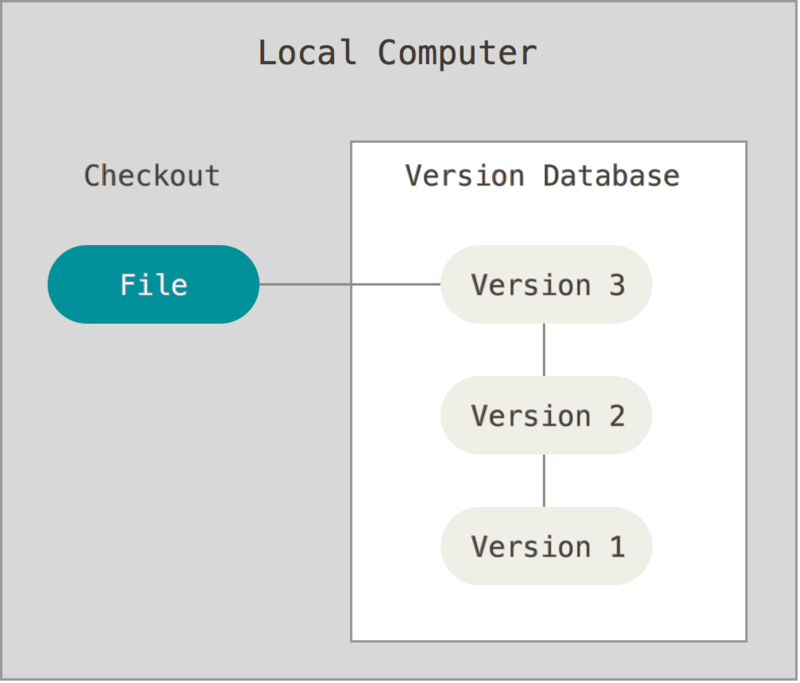
\includegraphics[width=\textheight]{local}
    \end{figure}
}

\frame[plain]{
    \frametitle{Gecentraliseerd}

    \begin{figure}[h]
    \centering
    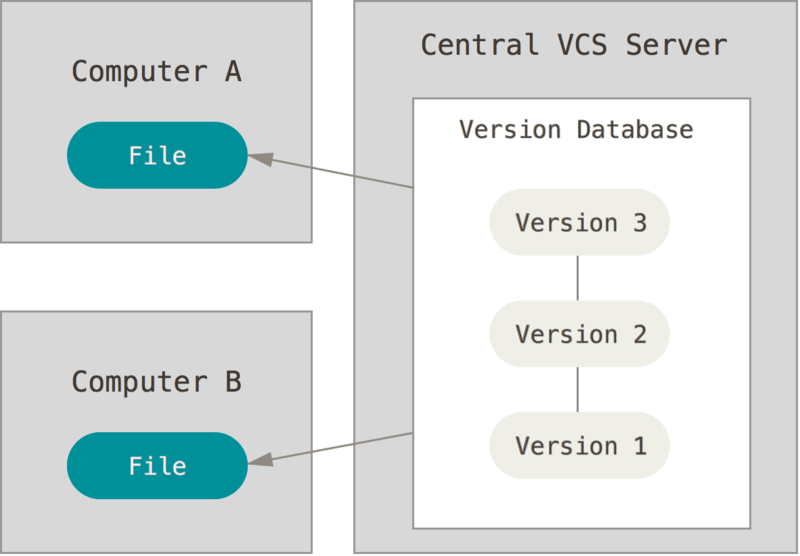
\includegraphics[width=\textheight]{centralized}
    \end{figure}
}

\begin{frame}
    \begin{itemize}
        \item \texttt{Concurrent Versions System (CVS)} (1986)
        \item \texttt{Subversion} (2000)
    \end{itemize}
\end{frame}

\frame[plain]{
    \frametitle{Gedistribueerd}

    \begin{figure}[h]
    \centering
    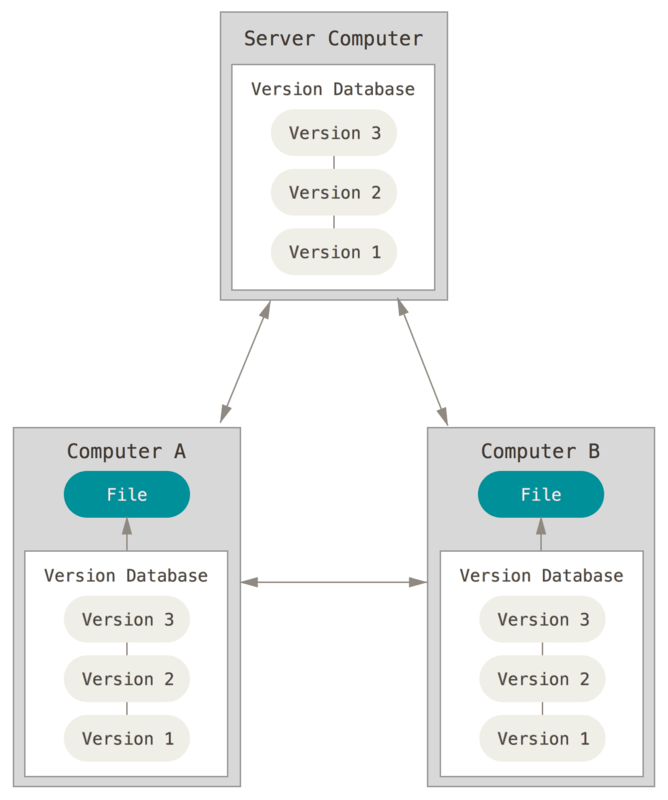
\includegraphics[width=0.8\textheight]{distributed}
    \end{figure}
}

\begin{frame}
    \begin{itemize}
        \item \texttt{BitKeeper} (2000)
        \item \texttt{Bazaar} (2005)
        \item \texttt{Git} (2005)
        \item \texttt{Mercurial} (2005)
    \end{itemize}
\end{frame}

\section{Git}

\subsection{Geschiedenis}

\frame[plain]{
    \begin{figure}[h]
    \centering
    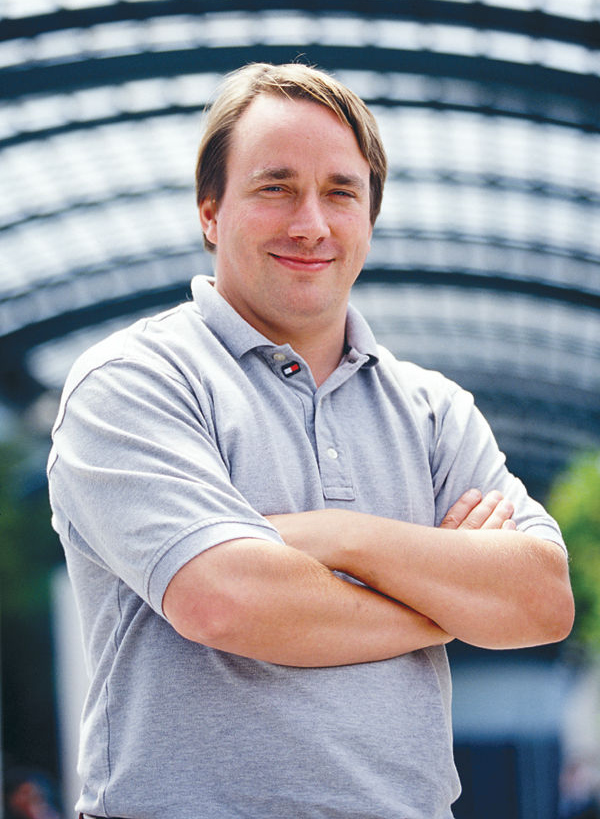
\includegraphics[width=0.7\textheight]{Linus_Torvalds}
    \end{figure}
}

\frame[plain]{
    \begin{figure}[h]
    \centering
    
\includegraphics[width=0.5\textheight]{Tux}
    \end{figure}
}

\frame[plain]{
    \begin{figure}[h]
    \centering
    
\includegraphics[width=0.5\textheight]{Git}
    \end{figure}
}

\subsection{Waarom Git?}

\begin{frame}
    \begin{itemize}
        \item Volledig gedistribueerd
        \item Goede ondersteuning voor niet-lineaire ontwikkeling
        \item Snelheid
        \item Efficiënt met grote projecten
        \item Gebruikersvriendelijk
    \end{itemize}
\end{frame}

\subsection{Hoe werkt het?}

\frame[plain]{
    \frametitle{Git denkt in momentopnames}

    \begin{figure}[h]
    \centering
    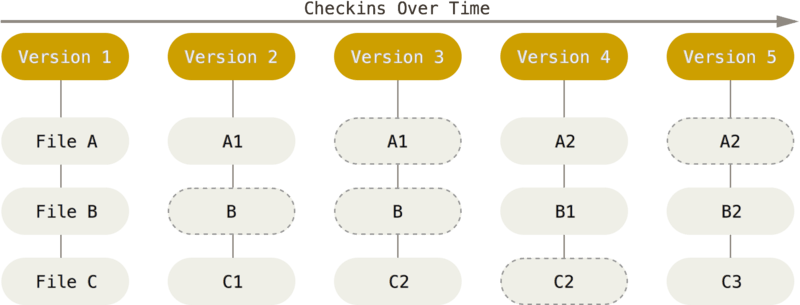
\includegraphics[width=\textwidth]{snapshots}
    \end{figure}
}

\frame[plain]{
    \frametitle{Integriteit}

    \begin{itemize}
        \item Alle objecten krijgen een checksum
        \item SHA-1
    \end{itemize}

    \vspace{10 mm}
    \pause
    \centering
    \texttt{b40508769cb0aac22d9f73c8669c3a13f5e9cf0b}
}

\frame[plain]{
    \frametitle{De drie toestanden}

    \begin{figure}[h]
    \centering
    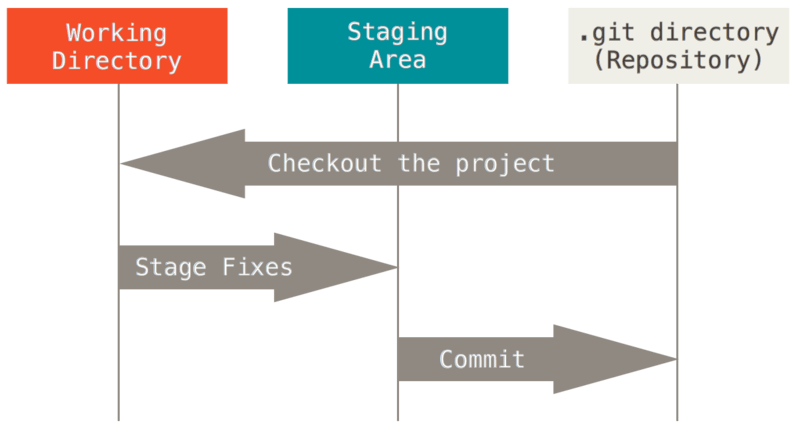
\includegraphics[width=\textwidth]{areas}
    \end{figure}
}

\begin{frame}
    \begin{itemize}
        \item De \texttt{git} commando-regel
        \begin{itemize}
            \item Geeft toegang to alle commando's
            \item Vereist basiskennis werken met Terminal
        \end{itemize}
        \pause
        \item Grafische tools
        \begin{itemize}
            \item Implementen maar een deel van de functionaliteit
        \end{itemize}
    \end{itemize}
\end{frame}

\section{Aan de slag}

\subsection{Installeren en configureren}

\begin{frame}[fragile]
    \frametitle{Installeren}

    \centering

    \begin{block}{Terminal}
    \verb/git --version/
    \end{block}

    \vspace{10 mm}
    \pause

    \url{https://git-scm.com/}
\end{frame}

\begin{frame}[fragile]
    \frametitle{Configureren voor gebruik}

    \begin{block}{Terminal}
\begin{verbatim}
git config --global user.name "John Doe"
git config --global user.email john@example.com
git config --global core.editor nano
git config --global color.diff true
\end{verbatim}
    \end{block}
\end{frame}

\begin{frame}[fragile]
    \frametitle{Hulp krijgen}

    \begin{block}{Terminal}
\begin{verbatim}
git help <commando>
git <commando> --help
man git-<commando>
\end{verbatim}
    \end{block}
\end{frame}

\begin{frame}
    \frametitle{Een Git repository verkrijgen}

    \begin{enumerate}
        \item Een repository initialiseren
        \item Een bestaande repository klonen
    \end{enumerate}
\end{frame}

\subsection{Een repository initialiseren}

\begin{frame}[fragile]
    \frametitle{Een repository initialiseren}

    \begin{block}{Terminal}
\begin{verbatim}
mkdir hello
cd hello
git init
\end{verbatim}
    \end{block}
\end{frame}

\frame[plain]{
    \frametitle{Wijzigingen vastleggen}

    \begin{figure}[h]
    \centering
    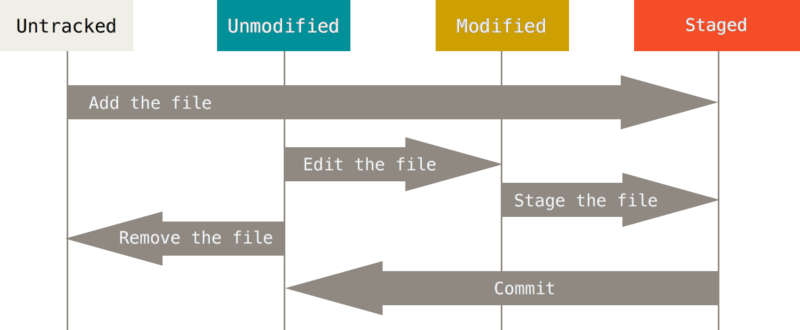
\includegraphics[width=\textwidth]{lifecycle}
    \end{figure}
}

\begin{frame}[fragile]
    \frametitle{De status controleren}

    \begin{block}{Terminal}
\begin{verbatim}
$ git status
On branch master
nothing to commit, working directory clean
\end{verbatim}
    \end{block}
\end{frame}

\begin{frame}[fragile]
    \frametitle{Bestanden toevoegen}

    \texttt{hello.py}
    \inputminted[bgcolor=monokaibg]{python}{source/hello.py}

    \vspace{10 mm}

    \begin{block}{Terminal}
    \verb/python3 hello.py/
    \end{block}
\end{frame}

\begin{frame}[fragile]
    \frametitle{De status controleren}

    \begin{block}{Terminal}
\begin{Verbatim}[fontsize=\tiny]
$ git status
On branch master

Initial commit

Untracked files:
  (use "git add <file>..." to include in what will be committed)

        hello.py

nothing added to commit but untracked files present (use "git add" to track)
\end{Verbatim}
    \end{block}
\end{frame}

\begin{frame}[fragile]
    \frametitle{Bestanden toevoegen en committen}

    \begin{block}{Terminal}
    \verb/git add hello.py/
    \end{block}
\end{frame}

\begin{frame}[fragile]
    \frametitle{De status controleren}

    \begin{block}{Terminal}
\begin{Verbatim}[fontsize=\scriptsize]
$ git status
On branch master
Changes to be committed:
  (use "git reset HEAD <file>..." to unstage)

      new file:   hello.py
\end{Verbatim}
    \end{block}
\end{frame}

\begin{frame}[fragile]
    \frametitle{Bestanden toevoegen en committen}

    \begin{block}{Terminal}
    \verb/git commit/
    \end{block}
\end{frame}

\begin{frame}[plain]
    \frametitle{Hoe ziet een goede commit message eruit?}

    \inputminted[fontsize=\scriptsize]{text}{source/commit-message.txt}
\end{frame}

\begin{frame}[fragile]
    \frametitle{De status controleren}

    \begin{block}{Terminal}
\begin{Verbatim}[fontsize=\scriptsize]
$ git status
On branch master
nothing to commit, working directory clean
\end{Verbatim}
    \end{block}
\end{frame}

\begin{frame}[fragile]
    \frametitle{Bestanden wijzigen en committen}

    \texttt{hello.py}
    \inputminted[bgcolor=monokaibg]{python}{source/hello2.py}
\end{frame}

\begin{frame}[fragile]
    \frametitle{Bestanden wijzigen en committen}

    \begin{block}{Terminal}
\begin{Verbatim}[fontsize=\tiny]
$ git status
On branch master
Changes not staged for commit:
  (use "git add <file>..." to update what will be committed)
  (use "git checkout -- <file>..." to discard changes in working directory)

        modified:   hello.py

no changes added to commit (use "git add" and/or "git commit -a")
\end{Verbatim}
    \end{block}
\end{frame}

\begin{frame}[fragile]
    \frametitle{Bestanden wijzigen en committen}

    \begin{block}{Terminal}
\begin{Verbatim}[fontsize=\scriptsize]
$ git diff
diff --git a/hello.py b/hello.py
index f7cf60e..5d97bdd 100755
--- a/hello.py
+++ b/hello.py
@@ -1 +1 @@
-print("Hello, world!")
+print("Hello, Git!")
\end{Verbatim}
    \end{block}
\end{frame}

\begin{frame}[fragile]
    \frametitle{Bestanden wijzigen en committen}

    \begin{block}{Terminal}
\begin{Verbatim}[fontsize=\scriptsize]
$ git add -p
diff --git a/hello.py b/hello.py
index f7cf60e..5d97bdd 100755
--- a/hello.py
+++ b/hello.py
@@ -1 +1 @@
-print("Hello, world!")
+print("Hello, Git!")
Stage this hunk [y,n,q,a,d,/,e,?]?
\end{Verbatim}
    \end{block}
\end{frame}

\begin{frame}[fragile]
    \frametitle{Bestanden wijzigen en committen}

    \begin{block}{Terminal}
\begin{Verbatim}[fontsize=\scriptsize]
$ git status
On branch master
Changes to be committed:
  (use "git reset HEAD <file>..." to unstage)

        modified:   hello.py
\end{Verbatim}
    \end{block}
\end{frame}

\begin{frame}[fragile]
    \frametitle{Bestanden wijzigen en committen}

    \begin{block}{Terminal}
\begin{Verbatim}[fontsize=\scriptsize]
$ git diff --staged
diff --git a/hello.py b/hello.py
index f7cf60e..5d97bdd 100755
--- a/hello.py
+++ b/hello.py
@@ -1 +1 @@
-print("Hello, world!")
+print("Hello, Git!")
\end{Verbatim}
    \end{block}
\end{frame}

\begin{frame}[fragile]
    \frametitle{Bestanden wijzigen en committen}

    \begin{block}{Terminal}
    \verb/git commit/
    \end{block}
\end{frame}

\begin{frame}[fragile]
    \frametitle{Commit geschiedenis bekijken}

    \begin{block}{Terminal}
    \verb/git log/
    \end{block}

    \pause

    \begin{block}{Terminal}
    \verb/git show <commit>/
    \end{block}

    \pause

    \begin{block}{Terminal}
    \verb/git blame <bestand>/
    \end{block}
\end{frame}

\begin{frame}[fragile]
    \frametitle{Commit ongedaan maken}

    \begin{block}{Terminal}
    \verb/git revert .../
    \end{block}

    \pause

    \begin{block}{Terminal}
    \verb/python3 hello.py/
    \end{block}
\end{frame}

\begin{frame}[fragile]
    \frametitle{Git repository resetten}

    \begin{block}{Terminal}
    \verb/git reset .../
    \end{block}

    \pause

    \begin{block}{Terminal}
    \verb/git log/
    \end{block}
\end{frame}

\subsection{Een bestaande repository klonen}

\begin{frame}[fragile]
    \begin{block}{Terminal}
    \verb$git clone https://github.com/libgit2/pygit2$
    \end{block}

    \pause

    \begin{block}{Terminal}
    \verb$git clone git@github.com:libgit2/pygit2.git$
    \end{block}
\end{frame}

\begin{frame}[fragile]
    \begin{block}{Terminal}
    \frametitle{De remote repository}

\begin{Verbatim}[fontsize=\scriptsize]
$ git remote -v
origin  https://github.com/libgit2/pygit2 (fetch)
origin  https://github.com/libgit2/pygit2 (push)
\end{Verbatim}
    \end{block}
\end{frame}

\begin{frame}[fragile]
    \begin{block}{Terminal}
    \frametitle{Branches}

\begin{Verbatim}[fontsize=\scriptsize]
$ git branch
* master
\end{Verbatim}
    \end{block}
\end{frame}

\begin{frame}[fragile]
    \begin{block}{Terminal}
    \frametitle{Branches}

\begin{Verbatim}[fontsize=\scriptsize]
$ git branch remove_todo

$ git branch
* master
  remove_todo

$ git checkout remove_todo
Switched to branch 'remove_todo'

$ git branch
  master
* remove_todo
\end{Verbatim}
    \end{block}
\end{frame}

\begin{frame}[fragile]
    \begin{block}{Terminal}
    \frametitle{Branches}

\begin{Verbatim}[fontsize=\scriptsize]
$ git checkout master
Switched to branch 'master'
Your branch is up-to-date with 'origin/master'.

$ git merge remove_todo
Updating 0f64ac4..685569e
Fast-forward
 TODO.txt | 16 ----------------
 1 file changed, 16 deletions(-)
 delete mode 100644 TODO.txt
\end{Verbatim}
    \end{block}
\end{frame}

\begin{frame}
    \frametitle{Een repository forken op GitHub}

    \begin{enumerate}
        \item Maak een GitHub account aan
        \item Genereer een SSH key
        \item Voeg de SSH key toe aan je ssh-agent
        \item Voeg de SSH key toe aan je GitHub account
        \item Fork deze repository op GitHub: \url{https://github.com/spereira-ct/git-intro}
    \end{enumerate}
\end{frame}

\begin{frame}
    \frametitle{De repository klonen}

    \begin{enumerate}
        \item Ga naar \url{https://github.com/spereira-ct/git-intro}
        \item Kloon de repository \textbf{met SSH}
        \item Maak lokaal een nieuwe branch aan in de repository
        \item Switch naar de nieuwe branch
        \item Voeg je naam toe onder ``Contributors'' in de \texttt{README}
        \item Commit je wijzigingen
        \item Merge je branch met de \textbf{master} branch
        \item Push de \textbf{master} branch naar \textbf{origin master}
        \item Ga naar \url{https://github.com/spereira-ct/git-intro} en check of je naam erbij staat
    \end{enumerate}
\end{frame}

\section*{Naslagwerk}

\begin{frame}{Naslagwerk}
    \begin{itemize}
    \item Officiële Git website: \url{https://git-scm.com/}
    \item Pro Git boek: \url{https://git-scm.com/book/}
    \item Hoe schrijf je een Git Commit Message: \url{https://chris.beams.io/posts/git-commit/}
    \item Meer Git tips: \url{http://gitready.com/}
    \end{itemize}
\end{frame}

\end{document}
